\chapter{General Introduction}

\section{Fruits and vegetable production challenges}

Fruits and vegetables are important sources of trace elements, vitamins, and minerals in human nutrition. The \gls{who} recommends consuming at least 400 grams of fruits and vegetables per day to prevent malnutrition (\url{https://www.who.int/news-room/fact-sheets/detail/healthy-diet}). For example, broccoli (\textit{Brassica oleracea} L.) heads, which are one of the most important components of the global vegetable market, have shown their great potential to prevent cancer and cardiovascular disease by several case studies \citep{mahn_overview_2012,latte_health_2011}. However, their supply and quality can be easily affected by extreme weather events (\url{https://www.bbc.com/news/business-64776969}). Moreover, climate change and global warming also have negative impacts on vegetables, especially lettuce and broccoli, which need a cold accumulation period to produce a harvest \citep{bisbis_potential_2018}. In addition, different field management practices (e.g., tillage, density, and nutrients) also affect vegetable yield and quality \citep{jackson_onfarm_2004, satodiya_effect_2015}. Hence, it is important to monitor the plants during their growth stages and make proper management decisions promptly to ensure vegetable supply and quality.

Conventional agricultural management activities for such purposes require significant manual labor and are now facing several challenges. Firstly, they often require professional knowledge and may be subject to human error. Secondly, the availability of human labor in agriculture is currently decreasing due to long-term global events, such as urbanization and aging populations, as well as short-term pandemics, such as economic recessions and \gls{covid19} \citep{gallardo_adoption_2018, larue_labor_2020}. As a result, there is an unprecedented demand for labor-saving technologies. The development of technologies, such as automation, sensing, big data analysis, computer vision, and artificial intelligence, has made it possible to address such demands and thereby spark the digital revolution in the agricultural industry \citep{gallardo_adoption_2018}.

\section{Plant phenotyping techniques}
% background introduction for plant phenotyping
The labor-saving and digitized plant status monitoring, also known as plant phenotyping, has been rapidly developed and implemented in recent years \citep{araus_field_2014}. It is defined as ``\textit{the application of methodologies and protocols to measure specific traits related to plant structure or function with traits ranging from cellular to whole-plant levels}'' \citep{fiorani_future_2013, ghanem_physiological_2015}. Although different workflows are required for different crops and applications, the general workflow of plant phenotyping can be summarized as follows: 1) Data collection, which collects plant data using various sensors; 2) \gls{roi} extraction, which detects or segments plant parts at expected levels (e.g., full canopy or single organ) from the collected data; and 3) crop trait calculation and guidance for practical applications \citep{zhao_crop_2019}.

\subsection{Data collection}
%% platform types -> indoor, outdoor(ground, aerial, satellite)
For data collection, there are various sensors available for different purposes in plant phenotyping. These sensors can be categorized as environmental sensors (e.g. light intensity, temperature, and humidity) and plant sensors (e.g. organic compounds and plant images) \citep{garlando_plants_2020}. Environmental sensors are typically fixed in place as part of the \gls{iot} system to record critical environmental factors that affect plant phenotypes \citep{ghanem_physiological_2015}. On the other hand, plant sensors are usually mounted on platforms and moved around, as shown in Figure~\ref{fig:int1}. These platforms enable data collection at different scales, from the organ level to the individual and canopy levels, as demonstrated in both indoor (Figures~\ref{fig:int1}a-d) and outdoor (Figures~\ref{fig:int1}e-k) settings.

\begin{figure}[htb!]
  \begin{center}
    \resizebox{\textwidth}{!}{
      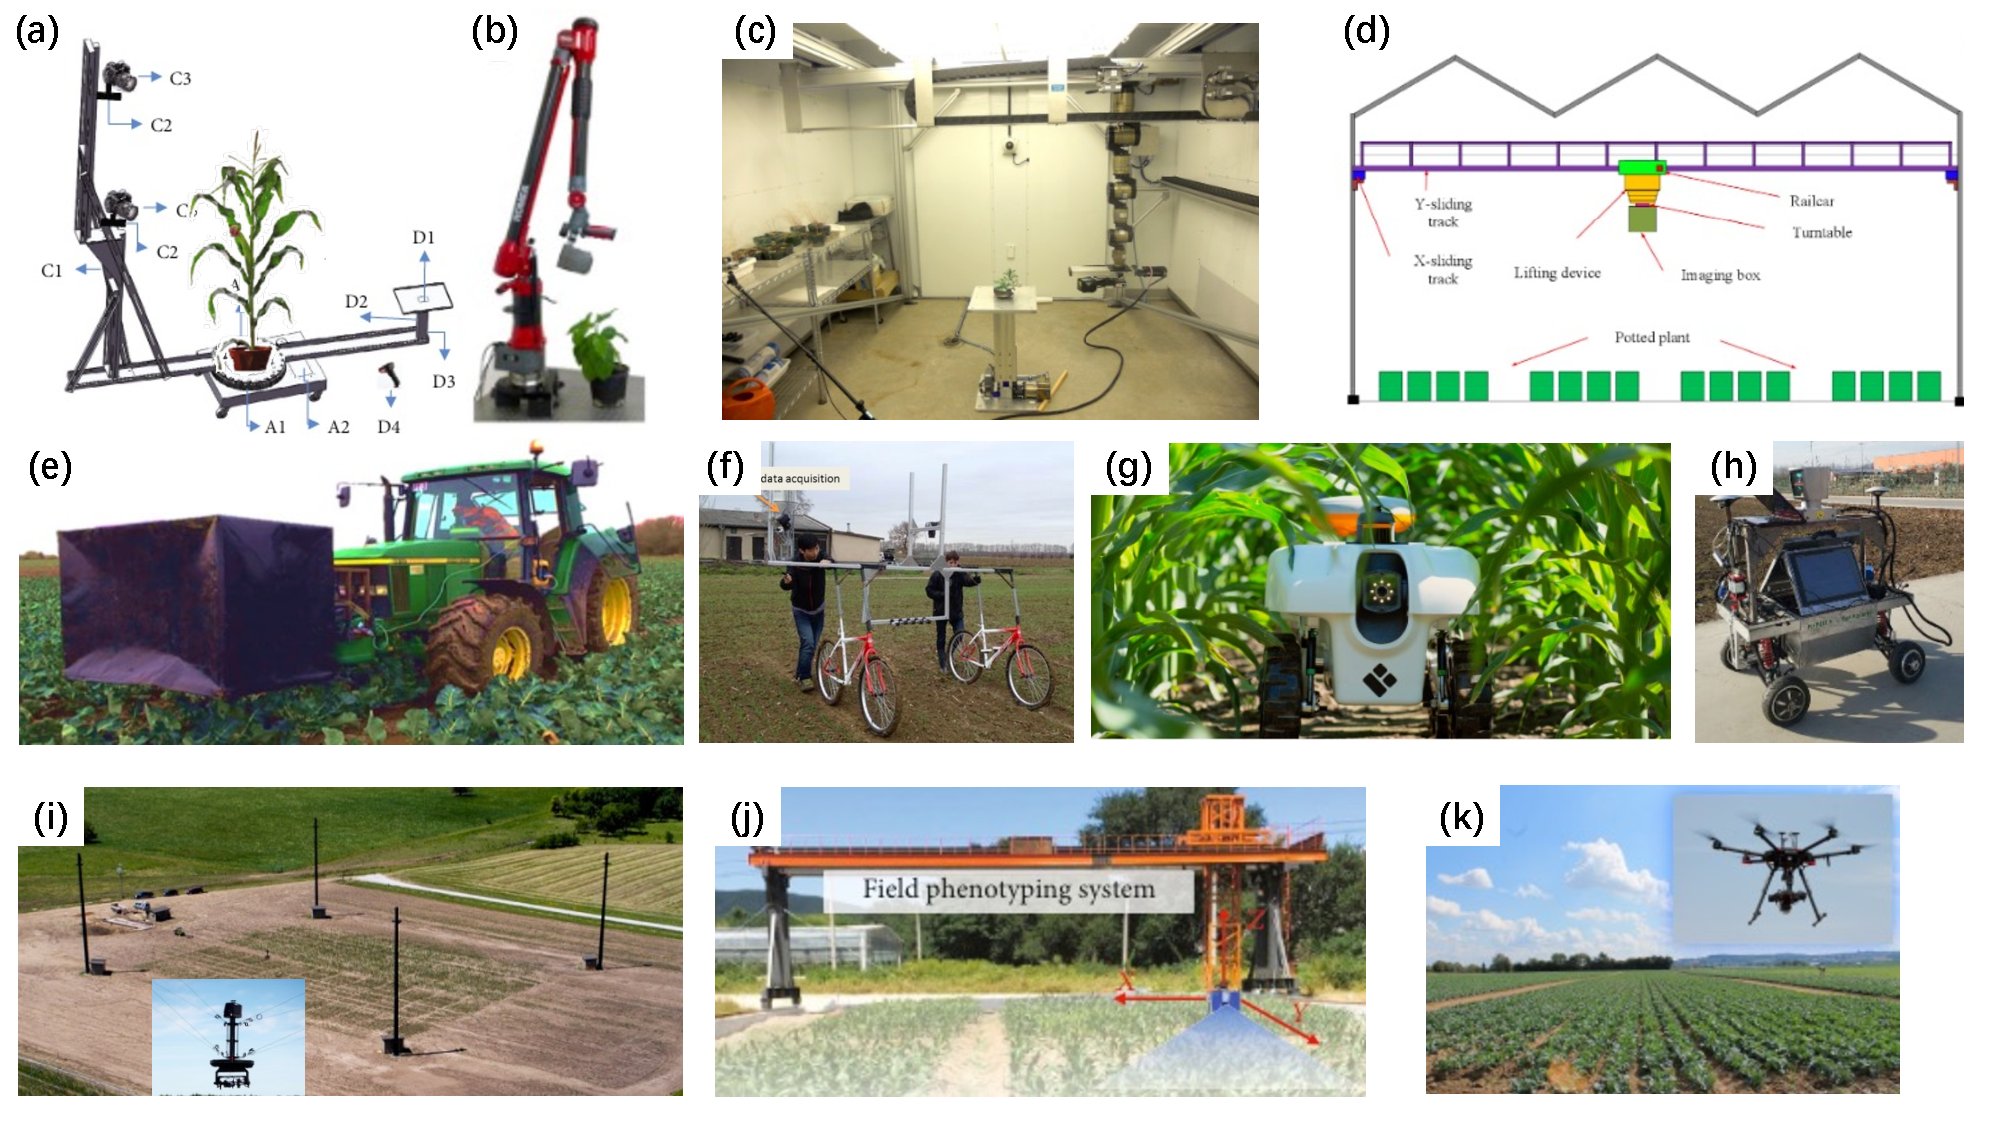
\includegraphics{figures/int/platforms.pdf}
    }
  \end{center}
  \caption[Example of platforms for plant phenotyping]{
    Example of platforms for plant phenotyping. (a-b) self-designed indoor devices \citep{wu_mvs-pheno_2020,schunck_pheno4d_2021}; (c-d) robotic arms in growth chamber or greenhouse \citep{chaudhury_machine_2018, du_greenhouse_2021}; (e) tractor \citep{kusumam_3d_2017}; (f) ground vehicle \citep{liu_estimation_2017}; (g-h) \gls{ugv} \citep{mcguire_high_2021, qiu_field-based_2019}; (i-j) robotic outdoor instruments \citep{bai_nu-spidercam_2019, jin_exploring_2021}; and (k) \gls{uav} \citep{kierdorf_growliflower_2022}
  }
  \label{fig:int1}
\end{figure}

% From the indoor to the outdoor, the commonly used platforms include self-designed indoor devices \citep{wu_mvs-pheno_2020,schunck_pheno4d_2021}, robotic arms in growth chamber or greenhouse \citep{chaudhury_machine_2018, du_greenhouse_2021}, tractor \citep{kusumam_3d_2017,blok_effect_2021}, ground vehicle \citep{liu_estimation_2017}, \gls{ugv} \citep{mcguire_high_2021,qiu_field-based_2019}, robotic outdoor instruments \citep{bai_nu-spidercam_2019, jin_exploring_2021}, \gls{uav} \citep{kierdorf_growliflower_2022, jang_review_2020}, and even satellite \citep{nguyen_monitoring_2020}. The scale of collected data using these platforms also changes from organ level, individual level to canopy level.

An important part of plant sensors is imaging sensors, which can record the morphological information of crops and are therefore commonly used in many plant phenotyping studies \citep{paulus_measuring_2019, feng_comprehensive_2021}. For example, infrared, multi- and hyper-spectral imaging sensors were used to calculate several vegetation indices \citep{han_modeling_2019}, such as \gls{ndvi}, to assess biomass \citep{jimenez-berni_high_2018}, yield, and water stress level \citep{herrero_yield_2020, romano_use_2011}, and to evaluate broccoli head freshness \citep{guo_evaluation_2022}. The common \gls{rgb} camera was also used to count plant number \citep{liu_estimating_2022}, plant density \citep{velumani_estimates_2021}, detect broccoli head \citep{blok_machine_2016}, and assess broccoli head quality \citep{stansell_use_2017}. These studies demonstrated the feasibility of using imaging sensors in plant phenotyping due to their high-efficiency and non-destructive nature.

%% 3D sensors
% introduction for 3D phenotyping, method to obtain 3D (passive, active) -> cost limit, choose RGB+SfM
However, these imaging sensors are difficult to use in directly describing the 3D morphological structure of plants, due to occlusion and dimension loss when projecting onto the 2D plane of photosensitive elements. As a result, inaccuracies and uncertainties arise when describing the 3D structure. With the development of sensing techniques, several studies have reviewed the latest available approaches for 3D plant phenotyping \citep{paulus_measuring_2019, okura_3d_2022, kochi_introduction_2021}. Figure~\ref{fig:int2} summarizes some of them, which are comprised of both active and passive scanners. A complete list of commercial 3D scanners is also provided by \citet[Table 5]{bartol_review_2021}.

\begin{figure}[htb!]
  \begin{center}
    \resizebox{\textwidth}{!}{
      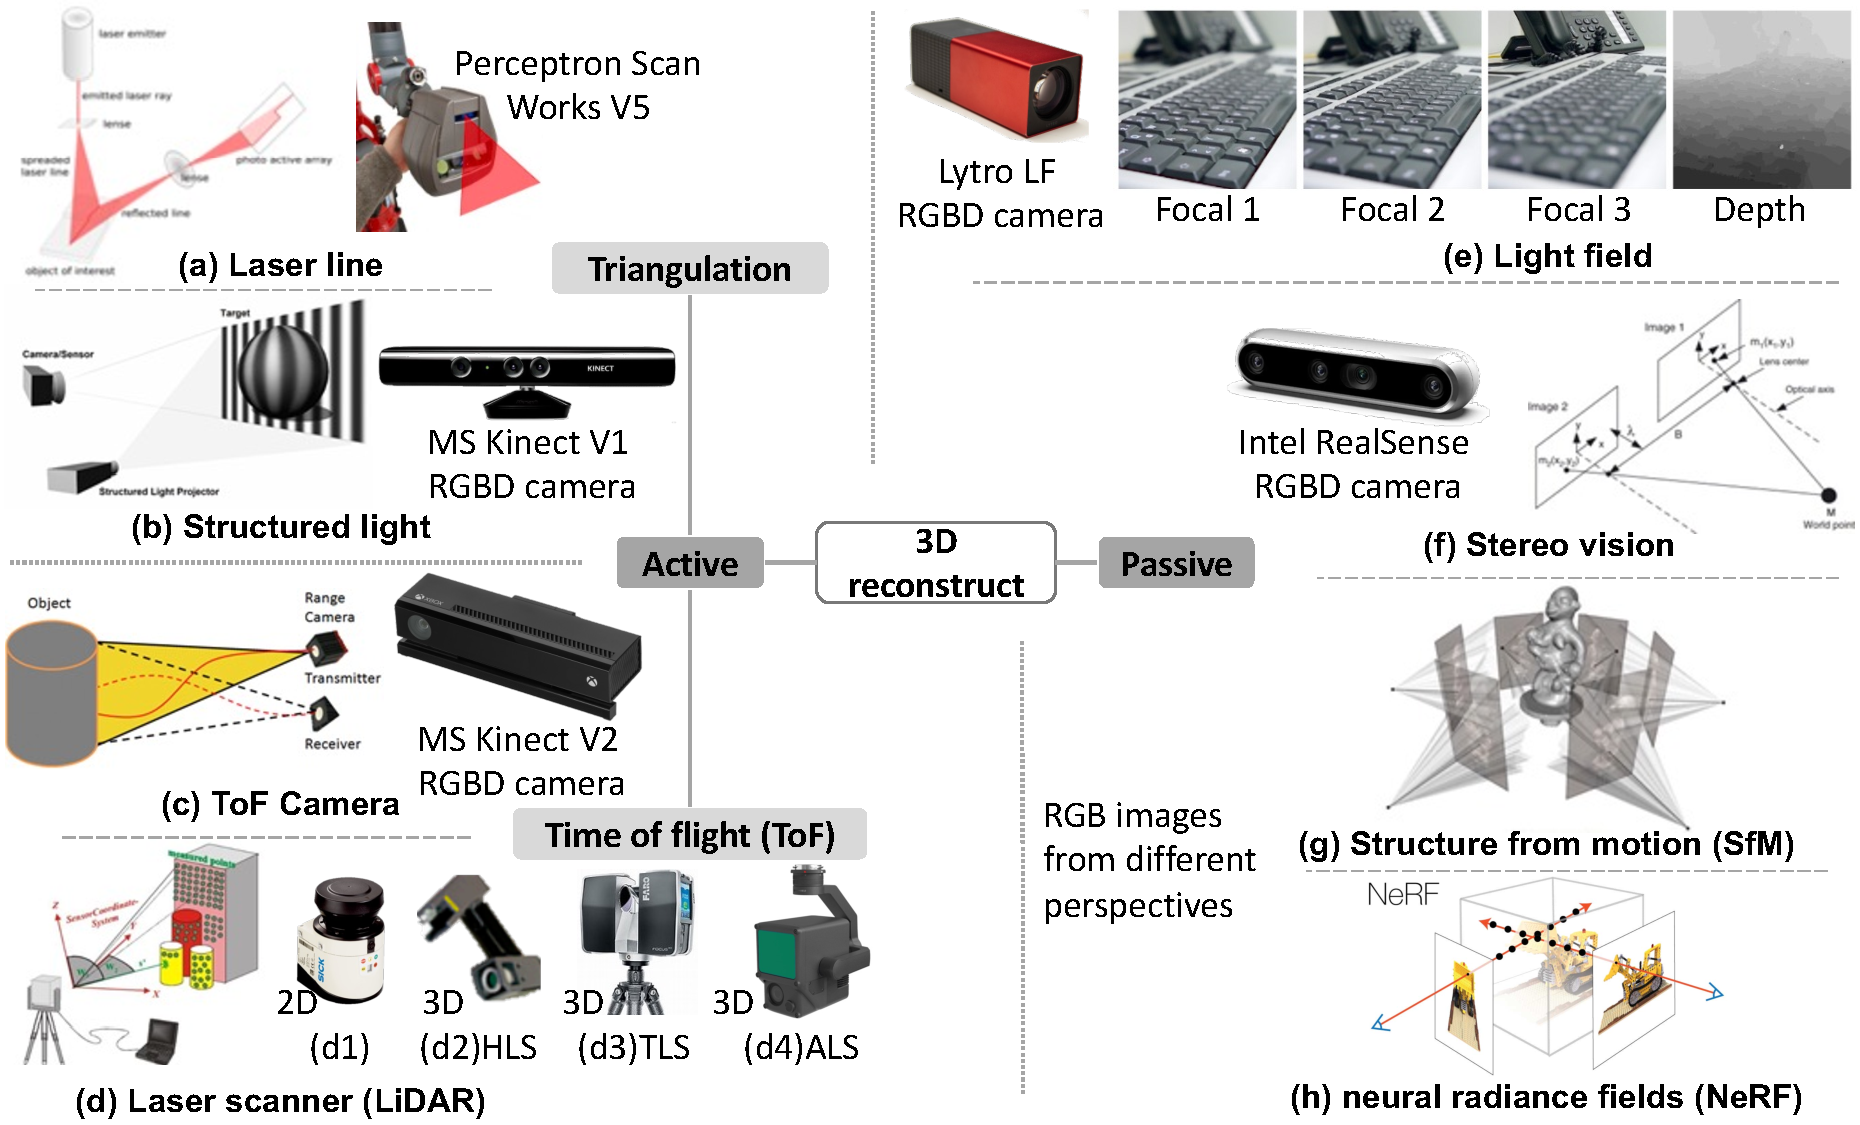
\includegraphics{figures/int/recons_sensors.pdf}
    }
  \end{center}
  \caption[Common methods for 3D structure reconstruction]{
    Common methods for 3D structure reconstruction. (a-d) The active sensors rely on projecting lights on the object and analyzing the reflection results, where (d) \acrfull{lidar}; (d2) \acrfull{hls}; (d3) \acrfull{tls}; (d4) \acrfull{als}; (e-g) the passive sensors rely on analyzing the passively received image groups. 
  }
  \label{fig:int2}
\end{figure}

The active scanners use a light source to project on the object and analyze the reflection results to obtain the structure. It consists of two main parts: triangulation and \gls{tof}. The triangulation approach uses the shape changes on the projected straight laser line(s) to obtain the object structure. For example, \citet[Figure~3]{schunck_pheno4d_2021} used a laser line (Fig.~\ref{fig:int2}a) triangulation scanner (Perceptron Scan Works V5, Perceptron Inc., USA) to build a public 3D model dataset for maize and tomato. Structured light improves efficiency by projecting an array of lines which is often visible or infrared light, rather than laser (Fig.~\ref{fig:int2}b). The Microsoft Kinect V1 is one of the famous \gls{rgbd} cameras based on this approach, which was released in November 2010. However, it was used in only a few plant phenotyping studies \citep{nguyen_structured_2015}. Since the release of the second version (Kinect V2, in July 2014) and the third version (Azure Kinect, in March 2020) with a different \gls{tof} approach and better performance \citep{tolgyessy_evaluation_2021, lachat_assessment_2015}. 
The \acrfull{tof} measures the distance between the sensor and points on the object to obtain its structure. Depending on the type of light source used, it can be divided into two categories: infrared for \gls{tof} cameras (Fig.~\ref{fig:int2}c) and laser for \gls{lidar} (Fig.~\ref{fig:int2}d). Since the sun is a massive source of infrared, infrared-based ToF cameras typically do not perform well in outdoor environments with intense sunlight \citep{tolgyessy_evaluation_2021}. Therefore, they are commonly used for indoor plant reconstruction applications \citep{martinez_low_2019, zhang_3d_2020, xu_global_2023}. In contrast, lasers are often more tolerant to sunlight due to their higher energy density, making them widely used in outdoor environments. There are different types of \gls{lidar} sensors used in 3D plant phenotyping applications. These include 2D \gls{lidar} scanners \citep{garrido_3d_2015}, 3D \gls{hls} \citep{ma_calculation_2019}, 3D \gls{tls} \citep{wu_accurate_2019, su_estimation_2018, qiu_field-based_2019}, and 3D \gls{als} \citep{ten_biomass_2019, nguyen_uav_2023}.

The passive scanners rely on analyzing passively received image groups, mainly using \gls{rgb} images. The light field camera takes a group of photos with different focal lengths, and the object structure is calculated according to different degrees of clarity caused by the different distances from the sensor (Fig.~\ref{fig:int2}e). For example, \citet{apelt_phytotyping_2015} built a light field camera system for measuring morphological traits related to plant growth. A commercial low-cost light field camera (Lytro LF, Lytro Inc., USA) was used as an \gls{rgbd} camera to monitor maize 3D morphological traits \citep{schima_imagine_2016}. Another commercial \gls{rgbd} camera, Intel RealSense L515(Intel Corporation, USA), uses a stereo vision approach (Fig.~\ref{fig:int2}f). It uses binocular vision like human eyes to obtain the object's structure. While for other RealSense models (D455, D435i, and D415) integrate the \gls{rgb} camera with \gls{lidar} \citep[Table 5]{bartol_review_2021}. \citet{blok_image_2021} used this RealSense \gls{rgbd} camera to estimate the broccoli head size with different degrees of occlusion, which is a tough problem for common \gls{rgb} cameras. The photogrammetry approach is based on \gls{rgb} images obtained from different perspectives (view angles) using common imaging sensors (Fig.~\ref{fig:int2}g). It first uses the overlapped area among images to estimate the camera poses and object's rough 3D structure (tie points), called \acrfull{sfm}. Then the \gls{mvs} is applied to densify the 3D point cloud of the tie points, and surface reconstruction and texture rendering are performed to obtain a 3D mesh model of the objects. For more details, please refer to \citet{hartley_multiple_2000} and \citet{snavely_scene_2010}.

% The structure from motion
%% software SfM
% ground sfm {Wu_MVS-Pheno_2020, Wang_Maize_2019, zhu_quantification_2020}; aerial sfm: {Liu_field-based_2021}
Unlike the previously mentioned scanners (Figures~\ref{fig:int2}a-f), which often require special, not-so-low-cost devices, the \gls{sfm} approach only requires an \gls{rgb} camera and \gls{sfm} software, with very flexible cost advantages. For the camera/sensor parts, even the cameras of smartphones at hand can be used to obtain photos for plant modeling \citep{li_measuring_2020}. If 3D plant models with ultra-high quality are required, a \gls{dslr} camera (over 4K resolution) can also be used to raise the 3D model quality to a higher level \citep{nguyen_3d_2016, drofova_use_2023}, often exceeding the resolution of previously commercial \gls{rgbd} cameras (around 1080p resolution). Meanwhile, a large number of \gls{sfm} open-source and commercial software packages are available for individual plants (close-range) and geo-referenced canopy (aerial) applications (Table~\ref{tbl:int1}). For this reason, many studies have used this approach to obtain 3D models of indoor individual plants \citep{wu_mvs-pheno_2020, zhou_automated_2019}, in-field individual plants \citep{jay_field_2015, herrero_structural_2023}, and in-field canopy \citep{kim_modeling_2018, herrero_canopy_2020}.

\begin{table}[htb]
  \caption[Softwares for 3D reconstruction using photogrammetry]{Softwares for 3D reconstruction using photogrammetry; ``Close-range'' is mainly used for building 3D models of individual plants or organs at the local coordinate; ``Aerial'' is mainly used for building geo-referenced canopy 3D models using \gls{uav} imagery with \gls{gps} coordinates.}
  \label{tbl:int1}
  % \begin{adjustwidth}{-0.05\textwidth}{-0.05\textwidth}
    \begin{center}
    % \resizebox{0.9\textwidth}{!}{
      \begin{threeparttable}
      \begin{tabular*}{\linewidth}{@{\extracolsep{\fill}} clcc}
        \hline
        \multicolumn{1}{c}{\textbf{Types}} & \multicolumn{1}{c}{\textbf{Software name}}                                                                      & \textbf{close-range} & \textbf{aerial}     \\ \hline
        Open source                        & AliceVision Meshrooms                                                                                           & $\checkmark$         & $\checkmark$        \\
                                           & COLMAP                                                                                                          & $\checkmark$         & $\checkmark$        \\
                                           & Multi-View Environment (MVE)                                                                                    & $\checkmark$         & $\times$            \\
                                           & OpenDroneMap\tnote{1}                                                                                           & $\times$             & $\checkmark$        \\
                                           & OpenMVG $\stackrel{2}{\rightarrow} \begin{cases} \text{MVE} \\ \text{OpenMVS} \end{cases}$                      & $\checkmark$         & $\checkmark$        \\
                                           & VisualSFM $\stackrel{2}{\rightarrow} \begin{cases}\text{MeshRecon}\\ \text{OpenMVS} \\ \text{PMVS} \end{cases}$ & $\checkmark$         & $\bigcirc$\tnote{3} \\
        Commercial                         & 3DF Zephyr                                                                                                      & $\checkmark$         & $\checkmark$        \\
                                           & Agisoft Metashape                                                                                               & $\checkmark$         & $\checkmark$        \\
                                           & Autodesk Recap Photo                                                                                            & $\checkmark$         & $\checkmark$        \\ 
                                           & ContextCapture                                                                                                  & $\checkmark$         & $\checkmark$        \\
                                           & Correlator3D                                                                                                    & $\times$             & $\checkmark$        \\
                                           & DJI Terra \tnote{4}                                                                                             & $\times$             & $\checkmark$        \\
                                           & DroneDeploy                                                                                                     & $\times$             & $\checkmark$        \\
                                           & Elcocision 10                                                                                                   & $\checkmark$         & $\checkmark$        \\
                                           & Pix4Dmapper                                                                                                     & $\times$             & $\checkmark$        \\
                                           & Reality Capture                                                                                                 & $\checkmark$         & $\checkmark$        \\ \hline
      \end{tabular*}
      \begin{tablenotes}
        \footnotesize
        \item[1] charges for a complied installer for whom is difficult to install from source code;
        \item[2] some software only provide \gls{sfm} pipeline, need to integrate them with \gls{mvs} software as a complete 3D reconstruction pipeline;
        \item[3] has video tutorials for processing UAV images, but no official documentation about making geo-referenced GeoTiff for common aerial products like \gls{dom} and \gls{dsm};
        \item[4] is optimized for DJI (Shenzhen DJI Technology Co., Ltd. China) drones only.
      \end{tablenotes}
      \end{threeparttable}
    % }
    \end{center}
  % \end{adjustwidth}
\end{table}

Recently, the \gls{cg} industry, which often needs to scan objects to create 3D models and render images from different perspectives, was introduced to a novel deep learning method by \citet{mildenhall_nerf_2022} (Fig.~\ref{fig:int2}h). The proposed approach, called \gls{nerf}, is based solely on the \gls{sfm} step and can bypass the time-consuming \gls{mvs}, 3D meshing, and 3D rendering steps required by photogrammetry. The official demo (\url{https://www.matthewtancik.com/nerf}) demonstrated the feasibility of obtaining plant 3D structures, and \citet{jignasu_plant_2023} obtained the maize 3D structure using this approach. However, the effectiveness of this approach relies on the quality of training data, and while there are many datasets available for industrial applications, there are not many for agricultural areas. As a novel technology, its application in agriculture still requires further development and thus is not included in this study.

% Considering the maturity of technology and the cost of sensors, the low-cost and mature photogrammetry approach (Fig.~\ref{fig:int2}g) has been chosen to collect research data in this study.

% \subsection{Data analysis for phenotyping}
% for data analysis.

\subsection{ROI extraction}

After collecting the data, the next step is to extract the \acrfull{roi} for further analysis. Different research purposes may have different interpretations of \gls{roi}. For canopy-level studies or breeding studies, the \gls{roi} refers to the regions within each plot boundary \citep{trevisan_htp_2020,han_drone_2021}. For individual-level studies, the \gls{roi} is the plant parts without any background such as soil or weeds \citep{ge_method_2019,guo_fieldbased_2020}. For organ-level studies, the \gls{roi} refers to the part of each organ without other parts of the plant, such as the broccoli head \citep{zhou_monitoring_2020} and sorghum tassel \citep{ghosal_weakly_2019} without leaves. This section summarizes different methods and algorithms for image analysis and 3D data analysis, including data processing, 2D-based image analysis from imaging sensors, and 3D-based point cloud analysis from 3D photogrammetry or \gls{lidar} scanner.

\subsubsection{Data preprocessing} \label{sec:prepro}

% plot region extraction (canopy level)
% easympe, other plot segments
For canopy-level or full-field phenotyping applications, the \gls{dom} is often used as the field plot map (by \gls{uav} photogrammetry); the 3D point cloud is often used as 3D canopy models (by \gls{uav} photogrammetry or \gls{lidar} scanner). However, processing the whole file image or 3D data directly is often impossible, since the file size of these whole canopy data is very large (often over 0.5GB and can reach 10GB+). One common data preprocessing step in plant phenotyping applications is to split the whole field into smaller parts \citep{wang_easyidp_2021}. It can be split into equal-size grids (e.g. \citet{bauer_combining_2019} split the full \gls{dom} image into several 250$\times$250 pixel grids) or by the boundary of each (micro) plot \citep{tresch_easympe_2019}. The latter option is more meaningful and often used.

To manually place plot boundaries and their labels on the \gls{dom} map, \gls{gis} software such as ArcGIS Desktop (Esri, Redlands, USA) or QGIS (open source \url{https://qgis.org}) is often utilized. (Micro) plot results are typically saved in shapefile format (*.shp) for better compatibility with other software. However, manually editing and operating software \gls{gui} can be time-consuming for large fields. Consequently, several studies have attempted to solve automatic \gls{roi} detection and generation by using computer vision. \citet{tresch_easympe_2019} developed an open-source Python package called EasyMPE for the semi-automatic generation and cropping of \gls{roi}. Subsequently, this tool was re-built using C++ by \gls{naro} and renamed PREPs (\url{http://cse.naro.affrc.go.jp/aitoh/PREPs}) for higher performance on the Windows platform. \citet{chen_grid_2020} also developed a Python-based tool called GRID (\url{https://zzlab.net/GRID}); \citet{mortensen_drone_2019} used MATLAB to create such a tool, and \citet{sara_automatic_2021} extended these tools by introducing the capability to slightly adjust the \gls{roi} location for better canopy fitting. All of these tools also support cropping the entire \gls{dom} into smaller parts within the \gls{roi} for post-processing.

For the 3D canopy point cloud, point cloud processing software such as MeshLab (open source, \url{https://www.meshlab.net}) or CloudCompare (open source, \url{https://www.cloudcompare.org}) is often used for similar tasks of cropping \gls{roi}, but it is not very convenient. Instead, it is more common to use the \gls{roi} shapefiles created in the previous step and write batch scripts for processing. For example, \citet{sun_field_2018} used a Matlab script to crop the \gls{roi} on \gls{lidar} point cloud, but they did not publish their code. Therefore, the EasyIDP python package was developed for easier processing of \gls{dom} and point cloud \citep{wang_easyidp_2021}. Even after segmenting the point cloud into smaller parts, point downsampling and noise removal are often necessary to reduce data size and processing difficulties due to the disorderliness of the point cloud's data structure \citep{ma_calculation_2019}.

After preprocessing the full field into smaller parts and data sizes, the following 2D- and 3D-based approaches can be applied to each part.

\subsubsection{2D-based approaches}

Most of the image analysis tasks for plant phenotyping can be summarized into three categories: classification, detection, and segmentation. The classification task involves determining the class of objects present in an image. For example, deciding whether a broccoli head is healthy or diseased \citep{garcia_towards_2021}. The detection task combines classification and localization to identify the kind of objects and their locations in an image. For instance, detecting the number of maize buds \citep{liu_estimating_2022} or sorghum tassels \citep{ghosal_weakly_2019} in an image. The segmentation task aims to separate an image into distinct regions with particular shapes and borders. It can be further divided into semantic segmentation (where a single label is assigned to all objects belonging to a particular class, e.g., all the regions of plants or broccoli heads in an image) and instance segmentation (where unique labels are assigned to each object, e.g., the regions of each broccoli head in an image). These tasks (classification, detection, and segmentation) are not independent of one another, as semantic segmentation often involves classifying each pixel to obtain the segmentation result of the entire image \citep{guo_easypcc_2017}, while instance segmentation usually requires combining the results of semantic segmentation and detection to identify each object's region \citep[see Fig.~2]{luling_using_2021}.

% [todo] a figure about broccoli detection, sematic segmentation, and instance segmentation.

%%% traditional CV method
The most conventional approach is to use computer vision algorithms on common \gls{rgb} images. In some simple cases, a manually defined color threshold can be used to separate plants from their backgrounds. For example, \citet{choudhury_holistic_2018} converted maize plant images from \gls{rgb} to \gls{hsv} and used ``\textit{hue (range 0.051-0.503), saturation (range: 0.102-0.804) and value (range 0.000-0.786)}'' to separate plant regions from the background. However, in most outdoor images with complex lighting and background conditions, manual thresholding does not perform well. Therefore, \citet{meyer_verification_2008} proposed color vegetation indices (NDI, ExG, and ExR) and combined them with \citet{otsu_threshold_1979} thresholding algorithm for automated crop imaging applications. To enhance compatibility with more complex scenarios and not be restricted to green plants, \citet{guo_easypcc_2017}  manually annotated the training data and trained machine learning classifiers based on extended color information. Additionally, \citet{zou_broccoli_2019} and \citet{blok_machine_2016} segmented broccoli buds and heads, respectively, using texture and color information and a trained \gls{svm} classifier.

%%% deep learning based method
%% -> 深度学习2D图像检测算法 siyuan
In the same way, deep learning techniques show great potential for achieving better results in \gls{rgb} image processing. The \gls{cnn} is a well-known deep learning framework for color imagery and has been used by many phenotyping studies. For instance, \citet{ghosal_weakly_2019} employed a pre-trained \gls{cnn} model to detect and count sorghum heads while \citet{liu_estimating_2022} used the Fast \gls{rcnn} to count maize seedlings. Additionally, \citet{bender_high_2020} used FastRCNN to detect and segment entire broccoli on \gls{rgb} images and shared them as public datasets. \citet{garcia_towards_2021} applied FasterRCNN to differentiate between immature and diseased broccoli. \citet{blok_effect_2021} simplified the MaskRCNN with data augmentation to improve broccoli head segmentation on \gls{rgb} images, but accuracy was affected by leaf occlusion. To address this issue, \citet{blok_image_2021} used \gls{orcnn} to recover the hidden head area.

% [todo?] convetional cv solution, but algriculutre also has many alternatives. (depth info, time-series info, hyperspectal)

\subsubsection{3D-based approaches}

Although 2D-based machine learning and deep learning approaches show the feasibility of extracting \gls{roi}s, for very complex scenes, it often requires labeling a considerable number of training sets to ensure better performance. The 3D-based approaches can not only provide more morphological information but also greatly simplify complex tasks.

The depth information is often used as a common and simple 3D-based approach. The depth image is a common file format for this information, which uses pixels to record depth values. It can be obtained from either depth cameras (often for close-range; the depth value is the distance from the object to the camera) or photogrammetry (often for aerial; the depth value is the height or altitude). Such information has been widely used for better plant segmentation for phenotyping studies. For close-range applications, \citep{luling_using_2021} used the depth image generated by photogrammetry and color information to segment cabbage instances. For aerial photogrammetry applications, \citet{guo_fieldbased_2020} segmented the plant area inside each \gls{roi} using the color and depth information from \gls{dom} and \gls{dsm}, respectively.

Another format for recording depth information is the 3D point cloud. Analyzing the 3D point cloud is also of great importance for the 3D-based approach. The general processing workflow for this analysis includes: 1) data preprocessing to decrease data size (see Subsection \ref{sec:prepro}); 2) semantic segmentation for separating foreground (plants) and background (soils, etc.); 3) instance segmentation of each plant for individual-level studies; and 4) instance segmentation of each organ for organ-level studies. The conventional methods are introduced first, followed by stepping to 3D-based deep learning approaches.

To perform 3D-based semantic segmentation between plants and backgrounds, color thresholding can be applied to 3D point clouds with colors as well as in the 2D-based approach. In \citet[Fig.~3]{xiao_image-based_2020}, a manually defined \gls{rgb} threshold ($R-G\geq7$) was used to separate plant points from backgrounds like shadow and soil points. The geometry relationship among points can also be used for segmentation. \citet{ge_method_2019} applied \gls{gmm} clustering to recognize the points of broccoli buds and removed noises using the \gls{knn} algorithm. Instead of extracting plant parts, \citet{garrido_3d_2015} used \gls{ransac} plane regression to identify flat ground points and removed them.

After performing 3D-based semantic segmentation of the plant part, the 3D-based instance segmentation to split each plant should proceed for individual-level studies. \citet{hofle_radiometric_2014} developed a region-growth method based on the local maxima in elevation to split each maize bud from semantic-segmented results. It shares a similar idea with the \gls{dbscan} clustering method, which several studies later used for maize \citep{lin_segmentation_2022} and cotton balls \citep{sun_3d_2020}. \citet{kusumam_3d_2017} segmented broccoli heads using the Euclidean clustering method and the \gls{svm} classifier on the 3D features, and \citet{montes_real-time_2020} further improved its efficiency to almost real-time.

Finally, studies at the organ-level require segmentation of each organ, especially for crops with complex morphological structures (such as maize and tomato). Different studies proposed solutions depending on the morphological characteristics of the crops or cultivars. For maize leaf segmentation, \citet{jin_stemleaf_2019} proposed an \gls{mnvg} algorithm, \citet{liu_canopy_2021} used skeletonization and region growth, \citet{wang_dfsp_2023} proposed a distance field-based segmentation pipeline, and \citet{miao_label3dmaize_2021} used optimal transportation distance and published an interactive segmentation tool (Label3Dmaize, \url{https://github.com/syau-miao/Label3DMaize}). For tomato stem and leaf segmentation, \citet{rossi_implementation_2022} proposed a complex but automated workflow using Matlab, which includes radius detection, sphere climbing, and phyllotaxy retrieving. \citet{helin_using_2023} proposed a t-distributed stochastic neighbor embedding segmentation method and demonstrated its feasibility on five different plants (hibiscus, maple, tomato, tobacco, and rosebush). Additionally, \citet{dutagaci_rose-x_2020} and \citet{schunck_pheno4d_2021} published annotated datasets for evaluating 3D plant organ segmentation methods.

One limitation of the conventional 3D-based analysis method, like the conventional 2D-based image analysis method mentioned above, is the necessity to develop specific algorithms based on the characteristics and objectives of different plants. Existing algorithms often have low compatibility with new crops and objectives. The 2D-based deep learning approach shows the possibility of changing the difficulty from specific algorithm development to training data annotation. But, unlike the well-structured 2D raster image data ($m \times n$ matrix, Fig.~\ref{fig:int3}b), it is difficult to apply neural networks directly to the 3D point cloud data with disordered structures (Fig.~\ref{fig:int3}d).



\begin{figure}[htb!]
  \begin{center}
    \resizebox{\textwidth}{!}{
      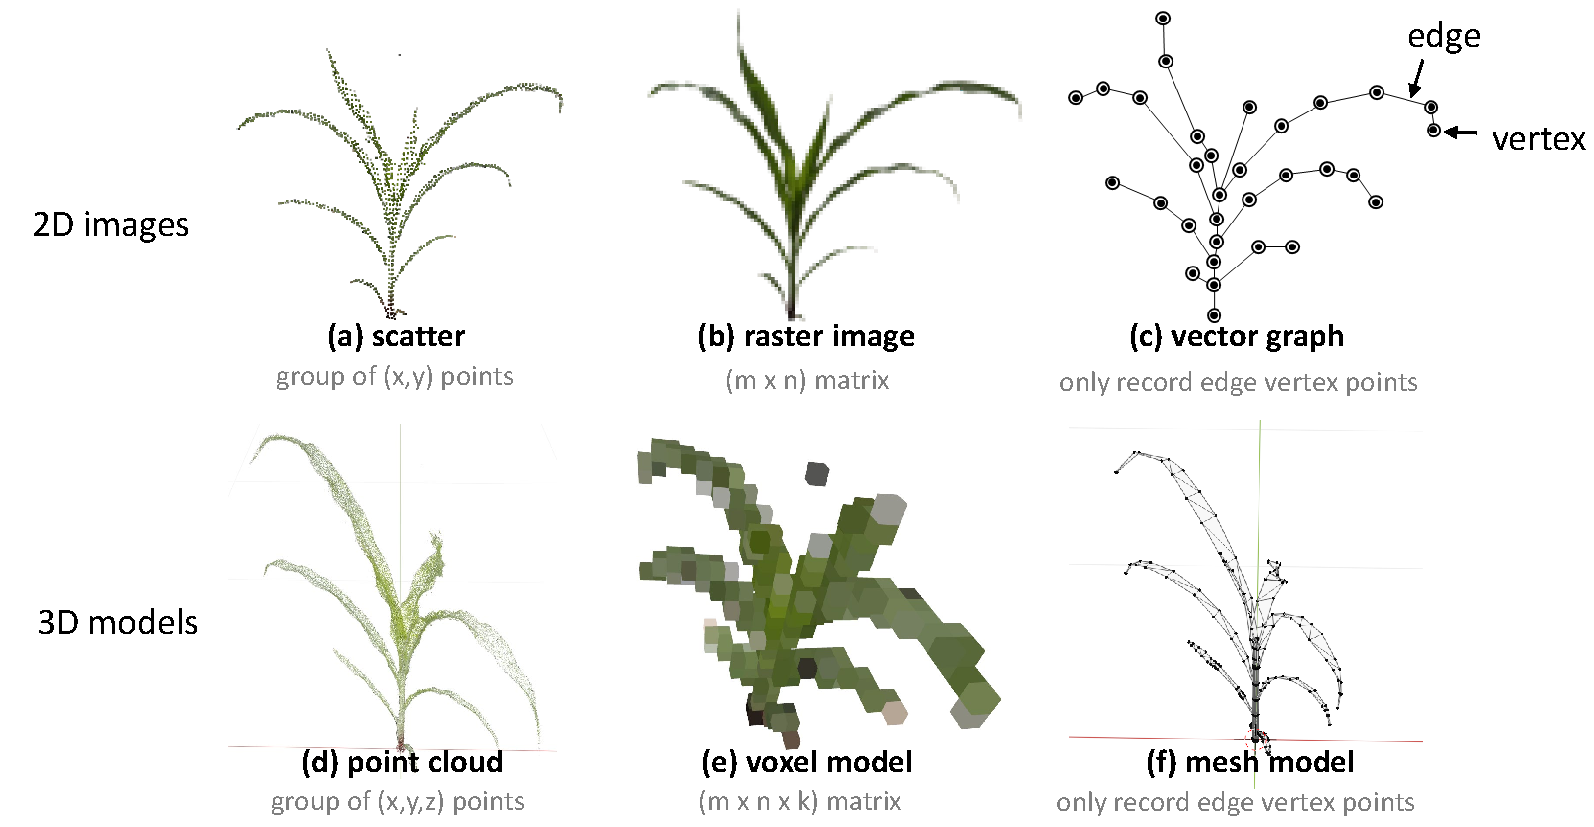
\includegraphics{figures/int/data_format.pdf}
    }
  \end{center}
  \caption[The compairson of 2D-based and 3D-based data format]{
    The comparison of 2D-based and 3D-based data format; (a) 2D point cloud also called scatter; (b) the common format for 2D images; (c) updated the scatter with relationship between points; (d) 3D point cloud, the most common format for 3D-based analysis; (e) the unit of 2D raster image is pixel, while the unit of 3D raster is voxel; (f) updated the point cloud with relationship, often used in \gls{cg} industry.
  }
  \label{fig:int3}
\end{figure}

Currently, there are four solutions for applying deep learning to the 3D point cloud. The first solution is 3D convolution, which converts the disordered point cloud (Fig. \ref{fig:int3}d) into the ordered voxel model (Fig.~\ref{fig:int3}e). One famous deep learning network based on this idea is VoxNet \citep{Maturana_VoxNet_2015}, but it is easily affected by the resolution (sidelength of the voxel) selection and is limited with small data sizes (maximum of $32 \times 32 \times 32$ voxel numbers). \citet{jin_separating_2020} developed a similar \gls{vcnn} for maize stem and leaf classification and segmentation.

The second solution is graph convolution, which converts the disordered point cloud into an ordered graph (Fig.~\ref{fig:int3}c\&f). The graph relationship already supports distinguishing different shape features like leaves (flat planes) and stems (long cylinders) according to self-defined rules \citep{mirande_graph-based_2022}. However, it is also possible to apply techniques such as \gls{gcn} \citep{wu_comprehensive_2021,zhou_graph_2020} or \gls{dgcnn} \citep{phan_dgcnn_2018} to the graph data. \citet{du_pst_2023} tested the feasibility of \gls{dgcnn} for instance segmentation on rapeseed leaves.

The third solution involves converting multi-view projections into 2D images for 2D-based detection or segmentation, and then re-projecting the results back to the 3D point cloud. One well-known network for this approach is the \gls{mvcnn}, which was proposed by \citet{su_mvcnn_2015}. \citet{jin_deep_2018} applied this method to segment individual maize plants from a 3D point cloud canopy. \citet{van_plant_2019} re-used the geometric relationship between 3D models and the raw images from photogrammetry to project the 2D deep learning results onto the raw images and back onto the tomato 3D point cloud models.

The last solution is to apply deep learning directly on the point cloud.  \citet{qi_pointnet_2016} first trained a deep learning network called PointNet by randomly shuffling the order of points in point clouds to avoid the impact of their order. However, the algorithm's complexity is factorial N, which becomes unacceptable for cloud sizes over 1000 points. Therefore, the PointNet++ \citep{qi_pointnet_2017} was proposed to solve the lack of hierarchical feature aggregation in the previous version. \citet{boogaard_boosting_2021} tested its feasibility on cucumber segmentation, and PointNet++ also serves as a comparison standard for several newly proposed networks for plants \citep{jin_separating_2020,zhou_automated_2022,du_pst_2023,li_psegnet_2022}. Specifically, \citet{zhou_automated_2022} and \citet{du_pst_2023} proposed \gls{pct}-based networks for broccoli head segmentation and rapeseed leaf segmentation, respectively. \citet{li_plantnet_2022} proposed a PlantNet and its updated version, PSegNet \citep{li_psegnet_2022}, for the organ segmentation of sorghum, tomato, and tobacco.

\subsection{Traits calculation}

After segmenting the \gls{roi}, several different kinds of trait calculations can be applied to obtain 2D-based and 3D-based results. \citet[Table 1]{du_greenhouse_2021} summarized the six categories of 2D-based traits obtained from common RGB images, namely: 1) geometric (morphological) traits, such as projected area, projected perimeter, convex area, convex perimeter, circumcircle diameter, the angle of the main axis, and the length of the long and short axis; 2) structure traits, such as the length or proportion of intersection line segments in concentric circles; 3) color space traits, such as the mean and variance of Red in RGB; 4) color index traits, such as \gls{exg}, \gls{vdvi}, \gls{rgri}; 5) color component traits, such as the 1st order color moment of B component; and 6) texture traits, such as contrast, dissimilarity, and homogeneity. Among these, geometric (morphological) traits, color index traits, and texture traits are commonly used in other studies. For example, \citet{stansell_use_2017} extracted texture traits like head color, head smoothness, head size, and head uniformity as broccoli head quality indices, while \citet{bauer_combining_2019} applied the color index trait \gls{ndvi} as an indicator of lettuce maturity.

When it comes to 3D-based approaches, besides the aforementioned 2D morphological traits such as projected canopy area, convex and concave hull area, canopy volume, and canopy height are also available for cotton canopy \citep{jiang_quantitative_2018}. For maize canopy applications, other canopy traits such as maize height \citep{hammerle_mobile_2018,qiu_field-based_2019} and row spacing \citep{qiu_field-based_2019} can also be calculated. \citet[Table 3]{jin_non-destructive_2020} calculated morphological traits of maize from canopy-level to leaf organ-level, including height, canopy cover, plant area index, projected leaf area, volume, stem diameter, leaf length, and width. \citet{itakura_automatic_2018} obtained the leaf inclination angle, and \citet{liu_canopy_2021} analyzed its effect on canopy light use efficiency. Additionally, 3D-based traits can also support advanced applications for drought stress \citep{su_evaluating_2019, sorrentino_lettuce_2020}, intercropping \citep{liu_field-based_2021} and light competition \citep{zhu_quantification_2020} analysis.

% [todo] skeleton extraction.
% \subsection{Advanced applications}
%% 时间序列分析的文献(使用时间序列追踪参数的变化) 思源笔记
% they were used for discovering the loci regulating flower opening [11\citep{han_drone_2021}].
%% 收期预测、光照模拟, 辅助QTL

\section{Challenges in plant phenotyping}

Despite the advances in phenotyping approaches, it is still challenging to apply them directly to the agricultural field. The reasons can be summarized as follows: 1) complex cultivation environments; 2) variations in crops and management; 3) the effects of occlusion; 4) the limitations of sensors; and 5) data processing.

% \subsection{Complex cultivation environments}
The complex weather conditions in the field often produce images with varying brightness and cloud shadows. Meanwhile, the in-field applications often have complex backgrounds with different soil textures and varying weeds. These factors pose great challenges to \gls{roi} detection and segmentation tasks. For some 3D-based approaches using the \gls{rgbd} cameras, the sun emits a massive amount of infrared radiation, and many infrared-based \gls{rgbd} cameras cannot perform well in such outdoor environments \citep{tolgyessy_evaluation_2021}. For the photogrammetry method, which assumes the object is solid from different angles, wind-caused leaf movement conflicts with that assumption and often results in the ghosting effect (double mapping), excessive pixelation, and seamline distortions in the final products \citep{duan_comparison_2017,lin_new_2021}. Even for the high-cost \gls{lidar} sensors using laser, dust particles and water droplets from rain and fog act as noise and affect the quality and accuracy of plant phenotyping applications. All of these environmental factors seriously impact the quality and accuracy of plant phenotyping applications.

% \subsection{Crop and management variations}
Different crop management practices can also lead to variations. For instance, planting methods can differ across farmlands, resulting in varying row spacings and plant densities. In fields with clear between-row intervals, a line detection method can be used to locate the position of each ridge and plot regions \citep[Fig.~1]{tresch_easympe_2019}. However, in fields lacking clear ridge intervals \citep[Fig.~3]{faye_toolbox_2016}, the line detection method may not be effective, necessitating the development of alternative approaches. Additionally, different cultivars of the same vegetable may exhibit distinct growth patterns and textures. For example, the application of different fertilizers to the same broccoli cultivar can impact head size and branch patterns \citep{nishida_estimation_2023}. The combination of these factors makes it challenging to develop a universal approach that can handle all scenarios. As a result, the typical approach is to create targeted algorithms for different crops and site characteristics, which can be time-consuming and heavily reliant on the expertise of computer science professionals.

% \subsection{Occlusion effects}
With the growth of plants, leaves can partially occlude vegetable fruits. For tomatoes \citep[Fig.~2a]{yamamoto_plant_2014} and grapes \citep[Fig.~1]{liang_segmentation_2022}, individual fruits can also occlude each other, resulting in plant structure loss in both 2D and 3D-based approaches. This can result in missed detection, and partial occlusion often leads to inaccuracies in area and other parameters. The issue of occlusion has become of great interest in the field of plant phenotyping \citep{blok_image_2021, boogaard_robust_2020, lehnert_3d_2019}.

% \subsection{Sensor limitation}
% image resoultion limites.
The sensor resolution is another limitation. Although most drone cameras now have a resolution greater than 4K and some drones even support attaching \gls{dslr} cameras for photography, considering the efficiency of surveys and the impact of the wind produced by the drone's propellers, the flying height is often above 10 $m$. This resolution is sufficient for surveys at the canopy scale, but it is difficult to achieve organ-level details. During the process of photogrammetry, the quality of the generated 3D product is influenced by the factors mentioned before and often decreases compared to the original image. Although the original image has better resolution than the photogrammetry-produced \gls{dom} and point cloud, it does not have the pixel-level \gls{gps} coordinates. This makes it impossible to accurately match plants from images to corresponding locations in the field.

% \subsection{Difficulties in data processing}
% 自动的模型的必要性
When applying machine learning for classification or regression tasks, model selection and tuning come also pose a challenge. \citet{wang_landscape_2019} reported that \gls{cart} outperformed \gls{svm}, \gls{rf}, and \gls{gbdt} on plant classification tasks. However, \citet{han_drone_2021} found that \gls{svm} performed best on flower classification tasks compared to \gls{rf}, \gls{cart}, \gls{lda}, and \gls{knn}. Furthermore, \citet{han_modeling_2019} reported that \gls{rf} yielded better results on biomass prediction than \gls{mlr}, \gls{svm}, and \gls{ann}. These studies indicate that the performance of different machine learning algorithms varies depending on the task at hand. From our experience, model selection is an empirical process that may require extra time to compare mainstream algorithms.

%% 数据集标注的工作量问题
% Besides, the model selection and parameter adjustment of machine learning as well as the training data preparation of machine learning, are still highly dependent on expert experiences and intensive labor. The auto machine learning framework and weakly supervised learning have merged as the interesting candidate to solve such dilemma.
Efficient acquisition of large amounts of high-quality image training data and annotations has become an urgent need for obtaining robust deep learning models in agriculture \citep{yang_applications_2021}. Many studies have attempted to solve these difficulties and their solutions can be summarized as follows: 1) decreasing the workload of training data annotation using automated annotation devices \citep{beck_embedded_2020}. However, reproducing such a system is challenging for researchers without a background in machinery, and it is also hard for outdoor applications; 2) publicly sharing datasets. For example, \citet{bender_ladybird_2019} shared a weekly scanned image dataset of cauliflower and broccoli, but without annotations. \citet{beck_weed_2020} shared the labeled weed seedling dataset collected by their automation system \citep{beck_embedded_2020}. \citet{david_global_2021} shared an extensive labeled wheat head dataset collected from 12 countries. However, current research is often distributed on various platforms with various label formats, making it cumbersome to use. The agricultural community urgently needs a standardized data-sharing platform; 3) use transfer learning to reduce the amount of required training data and time for model fitting \citep{yang_applications_2021}. \cite{desai_automatic_2019} used the ResNet-50 model pre-trained on the ImageNet dataset, while \citet{blok_effect_2021} used the Mask-RCNN model pre-trained on the COCO dataset. However, current models for transfer learning are trained on computer vision datasets, and \cite{blok_effect_2021} reported that broccoli in the CV datasets are dishes on plates, rather than broccoli grown in the field; 4) use data augmentation to generate a large number of annotations from small ones. \citet{zhou_monitoring_2020} used geometric transformations (random cropping and rotation), and \citet{blok_effect_2021} applied more geometric transformations and added photometric transformations to them. A more advanced data augmentation strategy involves generating fake images \citep{nesteruk_image_2021}. All these studies have shown that data augmentation can improve model performance; and 5) Use model-assisted labeling to significantly reduce the workload during data labeling. While some platforms provide model-assisted labeling, such as LabelBox (online, \url{https://docs.labelbox.com/docs/model-assisted-labeling}), v7labs (online, \url{https://www.v7labs.com}), and EISeg (offline, \url{https://github.com/PaddlePaddle/PaddleSeg}), they simply reduce the workload of training image annotation by using pre-trained models, rather than iteratively and interactively improving model performance for specific studies.

% 研究没有公布可用的代码,还需要重新复现。
Last but not least, reproducibility remains a problem in some phenotyping studies and tools. Many studies do not share their datasets or code publicly, making reproducibility difficult. This leads to a waste of resources in solving similar problems by reinventing the wheel. For studies that do share their codes or tools publicly, the application effect on other cultivars is often suboptimal. As \citet{lobet_image_2017} stated in the title ``\textit{Image Analysis in Plant Sciences: Publish Then Perish}'', many published phenotyping tools still suffer from severe reproducibility issues and a lack of ease of use. The main issues are: 1) code and example data are published on personal or laboratory websites and are often inaccessible due to slow download speeds caused by bandwidth costs and URL changes and the inability to maintain them; 2) only code files and straightforward introductory files are provided, with detailed instructions for setting up the code environment, runnable examples, and detailed API documentation often missing. This results in an inability to run and apply the code to their own data; and 3) a lack of follow-up maintenance and community support. Bugs may be solved through troubled email communications, but user experiences cannot be shared with other users.

\section{Research scope}

Broccoli (\textit{Brassica oleracea} L.) is an important crop for the global vegetable market that faces the aforementioned challenges. It grows in rows in the open field and has an uneven growth rate. As the cost of selective harvesting is still higher than one-time mechanical harvesting, deciding the optimal harvest date considering all head sizes is crucial for farmers. Aerial survey is one of the most efficient approaches to obtain full field information, but the broccoli head is often less than 20 cm, with different occlusions and positions, making the organ-level detection and segmentation of \gls{roi} challenging for current 3D plant phenotyping techniques. Furthermore, except for providing accurate statistical value for broccoli head size estimation, 3D virtual visualization may be more straightforward for farmers to make decisions.

% In this manuscript, the model selection and tuning part were completely taken over by auto-ml framework. After training data preparation, only 5 lines of python codes of auto-sklearn API were required to get the final well-trained model and feasible prediction results (Table 3 and Figure 6). With the assistant of auto-ml framework, researchers can focus more time on answering scientific questions rather than empirical model selection.

\section{Objectives of this study}

This Ph.D. thesis aims to improve the performance of 3D-based plant phenotyping on broccoli farmland using only low-cost \gls{rgb} cameras. To be more specific:

\begin{enumerate}
    \item To develop a semi-automatic close-range 3D reconstruction pipeline that can obtain high-quality 3D models of broccoli heads as a template database.
    \item To develop an unsupervised phenotyping data processing workflow that can automatically calculate several 1D to 3D morphological traits for close-range broccoli heads.
    \item To develop an improved workflow for aerial 3D reconstruction of broccoli canopy that can obtain better 2D morphological traits of broccoli heads in complex outdoor conditions.
    \item To automatically fuse the data between the close-range 3D database and the aerial canopy, which can calibrate the aerial-measured 2D morphological traits.
    \item To provide 3D virtual visualization for the head in the actual field.
    \item To publicly share all the codes used in this study (including the \LaTeX~code of this thesis) on Github, the most famous community for programming communication and bug reports, making this contribution free to use for anyone who has similar needs.
\end{enumerate}


\section{Outline of this study}

Chapter 1 provides an overview of the background information, related studies, and objectives of the study.

Chapter 2 presents the close-range 3D phenotyping pipeline, which obtains high-quality 3D models of destructively sampled broccoli heads. Firstly, an almost-automatic workflow that captures and saves the image of the target crop in multiple view angles is developed. Then, \gls{roi}s on the broccoli heads in the images are extracted by two pre-trained deep learning models. The preprocessed images are then fed into photogrammetry-based software (Agisoft Metashape) to generate 3D models using automatic processing scripts. Finally, the broccoli crown part is automatically segmented, the 3D model coordinates are corrected, and the phenotypic traits are calculated automatically. To evaluate the performance of the proposed pipeline, we compared some of the pipeline-measured traits with manually measured traits using the coefficient of determination and \gls{rmse}.

% which includes obtaining high-quality plant 3D models and calculating the 3D traits.
% the pipeline implementation for obtaining individual plant high-quality 3D structural models and calculating phenotypic traits. We made a full pipeline that can capture and save the image of the target crop in multiple view angles, then feed them to photogrammetry-based software and generate the 3D models, and finally calculate the phenotypic traits automatically. To evaluate the performance of the proposed pipeline, we conducted the experiments using the simple structure target (broccoli head) and complex structure target (container weeds). Statistically high correlations were observed between ground-truth measurements and pipeline calculated traits, including broccoli head size ($r^2>0.7$), weeds height ($r^2>0.95$) and projected leaf area ($r^2>0.95$). 

Chapter 3 presents the development of an aerial 3D phenotyping pipeline for \gls{uav} sensing on broccoli canopies. To overcome the challenges in distinguishing small broccoli heads on low-quality 3D canopy models from photogrammetry, we proposed a novel data-fusion method. This method allows for the segmentation of the broccoli head region on the original drone images (pixel coordinates without actual scale) and projective transformation of the results back to \gls{gps} coordinates to calculate actual size. We have used active learning and shoot-position guided regions to decrease the workload of deep learning data annotation. Manual measurements in the field were carried out to validate the accuracy of this pipeline.

% includes the 3D to 2D projection pipeline to improve deep-learning-based phenotyping

% The objective was to develop and validate the large-scale outdoor 3D phenotyping pipeline using drones equipped with commercial-level \gls{rgb} cameras. To overcome challenges in distinguishing the small broccoli heads on low-quality canopy 3D models, we proposed a novel method to segment broccoli head region on the original drone images, then trace results back on the canopy 3D model to calculate actual size traits. Good correlations (0.57<r2<0.74) between field-measured traits and pipeline-calculated traits were observed.
% This pipeline was then extended to estimate the optimal harvest date with the highest profit and maize canopy advanced traits by other lab members.

Chapter 4 tests the idea of data fusion for broccoli based on the pipeline built in Chapters 2 and 3. The piecewise affine transformation is used to locate the head segmentation regions more precisely in the \gls{gps}  coordinates than in Chapter 3. Then, automatic machine learning is used to calibrate the 2D morphological traits for each broccoli head from the aerial pipeline (Chapter 3) using the destructively sampled broccoli heads. Later, a modified normalized cross-correlation template matching method is used to find the closest broccoli head in the template database (Chapter 2) and transform it back to the aerial 3D canopy model for virtual visualization.

Chapter 5 summarizes the study's general conclusions and discusses potential future research prospects.

% short The close-range 3D reconstruction along with the pre-trained deep learning technique was used to build an ultra-high-quality broccoli 3D head model database. Then, the active learning approach and fused the data between 2D raw \gls{uav} image and 3D photogrammetry outputs were used to improve the accuracy and labor cost for aerial data analysis. Lastly, an automatic machine learning and template-matching method were used to fuse the data between the close-range database and the aerial field, which can provide a 3D virtual visualization for the head in the actual field.

% using the 3D to 2D projection and labor-saving active learning technique, 